
\documentclass[10pt,a4paper]{article}
\usepackage[utf8]{inputenc}
\usepackage[T1]{fontenc}
\usepackage{amsmath}
\usepackage{amsfonts}
\usepackage{amssymb}
\usepackage{graphicx}
\usepackage[version=4]{mhchem}
\usepackage{tikz}
\usepackage{pgfplots}
\pgfplotsset{compat=1.18}

\title{graphical functions}
\begin{document}

\begin{tikzpicture}
  \begin{axis} [xmin=-10, xmax=10,
                ymin=-10, ymax=10,
                axis x line=middle,
                axis y line=middle,
                xlabel = \(x\),
                ylabel = {\(f(x)\)},
                ]

    \addplot[color=red][domain=-5:5]{x^2};
    \addplot[domain=-10:10]{x+2};

\end{axis}
\end{tikzpicture} \\

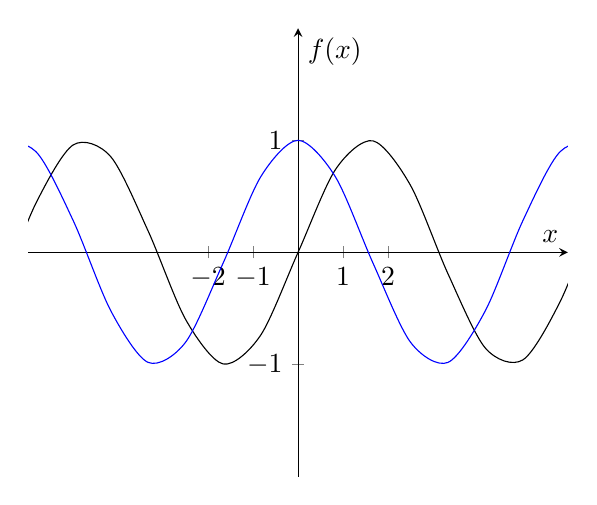
\begin{tikzpicture}
  \begin{axis} [xmin=-6, xmax=6,
                ymin=-2, ymax=2,
                xtick={-2,-1,0,1,2},
                ytick={-1,1},
                axis x line=middle,
                axis y line=middle,
                xlabel = \(x\),
                ylabel = {\(f(x)\)},
                ]

    \addplot[domain=-10:10,smooth] {sin(deg(x))};
    \addplot[domain=-10:10,smooth,color=blue] {cos(deg(x))};

\end{axis}
\end{tikzpicture}

\end{document}
